\apendice{Plan de Proyecto Software}

\section{Introducción}

Para todo proyecto que se va a producir, es fundamental realizar un estudio acerca de cuales son los los objetivos que se quieren alcanzar, en cuanto tiempo y que recursos se disponen para ello.
En este apartado se va a tratar sobre este establecimiento de metas y la temporalización de las mismas utilizando dos apartados principales:
\begin{itemize}
    \item Planificación temporal
    \item Estudio de viabilidad
    \begin{itemize}
        \item Viabilidad legal
        \item Viabilidad económica

    \end{itemize}

\end{itemize}


Debido a que se han utilizado metodologías ágiles durante el desarrollo de este proyecto, desde un inicio ha quedado muy claro cómo se gestionaban las tareas a realizar para poder ir generando un aporte de valor continuo tal como se muestra en la zona de planificación temporal.

Por otra parte, en el estudio de viabilidad se van a comentar tanto los aspectos económicos que conciernen al buen desarrollo del proyecto como las leyes que se necesite cumplir para tener garantizado que en un futuro no aparezcan inconvenientes legales

\section{Planificación temporal}


\subsection{Primer sprint 29-11-2023 / 20-12-2023}
Como primeros pasos para la creación del proyecto, se realiza un estudio inicial para considerar cuales van a ser los lenguajes de programación utilizados durante el proyecto. Debido a mi poca experiencia diseño web, opto por utilizar el framework de python \href{https://flask.palletsprojects.com/en/3.0.x/}{Flask} ya que de una manera sencilla me permite crear páginas web en un lenguaje de programación ya trabajado durante la carrera y tener una integración sencilla entre backend y frontend. Además de esta elección, en esta tarea se realizan labores de investigación y lectura de documentaciones para iniciar el proyecto con las habilidades suficientes para empezar a dar pequelos pasos en el diseño web.

Como otra tarea a realizar durante esta milestone, se determina como idea inicial obtener los datos a través de la realización de peticiones a una API . Esto permitía una manera simple de obtener unos datos alojados en internet y poder generar un filtro  para obtener el resultado esperado.
Tal como se menciona en la memoria, se inclina la balanza a favor de la API de Google, por lo que inicio la lectura de documentaciones para informarme como realizar las llamadas a este servicio.

Mientras se realizan esas tareas se toman apuntes para incluir la información de la API en la memoria.

Tras definir las tareas a realizar en este sprint, se estima que la duración de la realización de las tareas son de 10 horas, pero finalmente las tareas se completan en 7 horas.

\subsection{Segundo sprint 20-12-2023 / 16-01-2024}

Tras tomar las decisiones iniciales del anterior sprint, comienzo a investigar la estructura del Framework y los lenguajes HTML y CSS realizando pequeños ejercicios , ya que mi experiencia anterior con estas herramientas era muy limitada.

Una vez realizada esa toma de contacto  creo una ejemplo inicial de como podría estructurarse la web para debatirlo en la reunión de fin de sprint.
Para este inicialmente creo un catálogo básico  con una base de datos que permite realizar estas operaciones de manera manual:

\begin{itemize}
    \item Barra de navegación que permite cambiar de página.
    \item Sistema de Login para gestionar la aparición de botones ocultos.
    \item Consultar todos los libros existentes en la base datos.
    \item Realizar búsquedas de los libros existentes en la base de datos en base al título o al ISBN.
    \item Agregar un libro a la base de datos.
    \item Editar un libro de la base de datos.
    \item Eliminar un libro de la base de datos.

\end{itemize}

El sistema de Login se estableció para no permitir que ningún usuario que no tuviese credenciales pudiera realizar modificaciones de la base de datos. En el caso de que ejecutaran la URL exacta de la función, la protección de seguridad les llevaría a la pantalla de Inicio de Sesión.

\begin{figure}[h]
    \centering
    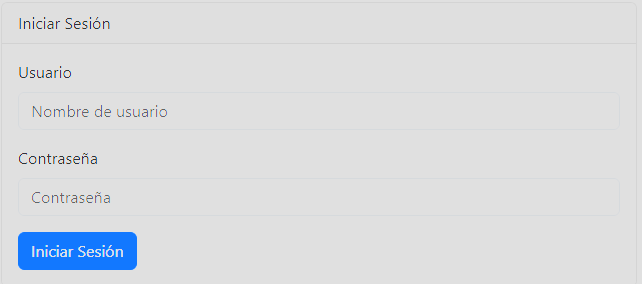
\includegraphics[width=0.9\textwidth]{Imagenes/Inicio_Sesion.png}
    \caption{Inicio de sesión}
    \label{fig:Inicio de sesión}
\end{figure}

Para poder tener más libertad de elementos para integrar dentro de la web, se decide utilizar la biblioteca Bootstrap 5, la cual tiene elementos predefinidos con estilos, generando una programación más eficiente y limpia.

Mientras continuo realizando apuntes para incluirlos en la memoria posteriormente.

Realizar estas tareas tuvo una estimación inicial de 45 horas, pero finalmente fueron 40 horas.

\subsection{Tercer sprint 16-01-2024 / 30-01-2024}

Una vez presentado y debatido este primer prototipo de página web en el Sprint, se decide continuar de esta base agregando más elementos para añadirle funcionalidades. De manera adicional, se comienza a realizar un prototipo web para ir documentando el esquema de secciones existente en este proyecto. Tal como se comenta en la sección de Técnicas y Herramientas,  el prototipo web se realiza con el programa Justinmind.

Además, se agrega otra funcionalidad considerada como esencial, una página que al seleccionar el libro te muestre toda la información disponible en la base de datos para todo usuario interesado en obtener datos.
Para ello, en cada libro mostrado en el catálogo se pone a disposición un botón que te redirige a esta página.

Durante esa reunión se propone la idea de incluir un apartado especifico para los administradores que permite importar y exportar en un archivo CSV todos los datos de cada libro contenidos en la base de datos. 
Esta idea se concibe principalmente por dos grandes motivos
\begin{itemize}
    \item Tener la oportunidad de volcar datos más rápido desde el archivo CSV y posteriormente cargar el contenido del fichero en la base de datos.
    \item Poder tener un duplicado de la base de datos por si el contenido de la misma quedase inaccesible o se realizara un cambio indeseado, lo cuál se solucionaría restableciendo el catálogo con el archivo de seguridad descargado.



\end{itemize}


\subsection{Cuarto sprint 30-1-2024 / 13-02-2024}
En este sprint se corrigieron un error relativo a la implementación de la importación y la exportación
El error consistía en que un administrador pudiera colocar el signo "," para separar dos elementos como por ejemplo dos ISBN o que se encontrase en el contenido de la descripción del libro, lo cual generaba errores a la hora de transformar los campos a columnas al tener ese mismo signo como delimitador. Por ese motivo se propuso la idea de cambiar el delimitador por defecto a el signo ";".

Tras realizar estas correcciones de errores iniciamos el proceso de obtener la información  de los libros de forma automática Aunque de manera inicial se valoró la opción de utilizar únicamente la API de Google Books,  se consideró interesante para  dar más fuentes de información y aumentar la dificultad técnica del proyecto la utilización de Web scraping. 
El  web scraping realizado se aplica sobre 2 páginas web las cuales tienen un catálogo de libros muy amplio. Estas webs son \href{https://www.amazon.es/}{Amazon} y \href{https://www.agapea.com/}{Agapea}. Estos tres proveedores nos permiten que en base a un ISBN o un Título, internamente se lancen unos procesos que busquen en los proveedores con las diferentes técnicas mostradas para que se pueda seleccionar el proveedor que nos de la información más precisa. 
En el caso de que se quisiera agregar un libro automáticamente pero se desee personalizar y usar una mezcla de los 3 proveedores, se dispone de un sistema de desplegables que nos permite realizar esta acción.

Durante el desarrollo en este espacio de tiempo, se considera que sería necesario implementar un sistema que nos permitiese proteger el catálogo de una importación que pueda encontrarse corrupta o con datos erróneos.
Por lo que antes de realizar la importación, aparece una ventana modal que recuerda al usuario que debería de exportar el catálogo actual por seguridad.

Para este sprint se estimo inicialmente unas 30 horas pero finalmente se realizó en 35.

\subsection{Quinto sprint 13-02-2024 / 27-02-2024}
Tras hacer las pruebas pertinentes de que la técnica de Web scraping es satisfactoria en y una gran mayoría de casos devuelve el libro correcto, (Los casos en los que falla es debido a la inexistencia de ese título en el catálogo de la plataforma en la que se busca), se pone como tareas en este sprint integrarlo a la página web en un apartado específico de búsqueda automática y acompañarlo de la llamada a la API de Google books. Para indicar al usuario que se esta ejecutando la búsqueda de libros, se añade una animación de carga.

Finalmente se pone como tarea el tratamiento de los datos obtenidos de esas fuentes, indicando con botones cual de los resultados de las fuentes es el deseado para agregar al catálogo.
En el caso de que se quisiera agregar un libro automáticamente pero se desee personalizar y usar una mezcla de los 3 proveedores, se dispone de un sistema de desplegables que nos permite realizar esta acción.

Durante el desarrollo en este espacio de tiempo, se considera que sería necesario implementar un sistema que nos permitiese proteger el catálogo de una importación que pueda encontrarse corrupta o con datos erróneos.
Por lo que antes de realizar la importación, aparece una ventana modal que recuerda al usuario que debería de exportar el catálogo actual por seguridad.

Este sprint recibió una estimación inicial de 30 horas pero se completaron todas las tareas en 20 horas.

\subsection{Sexto sprint 27-02-2024 / 2-04-2024}
En la reunión de inicio de este sprint se presentó la idea acerca de la posibilidad de cambiar la parte de frontend hasta ahora implementada utilizando Flask a un framework más potente llamado Angular. Esto se debe a que durante mis prácticas curriculares obtuve conocimientos de este framework, que además de utilizar HTML y CSS utiliza TypeScript para el desarrollo de las aplicaciones.
Tras hablarlo decidimos que este sprint se dedicaría a investigar la viabilidad de una refactorización completa del frontend a Angular mientras se realizaban desarrollos en la aplicación ya creada. 
De manera adicional, para poder realizar un intercambio de información óptima el backend de Flask tendría que modificarse para convertirse en una API. Por lo que se realizó este estudio también.

Como desarrollo en paralelo en la aplicación actual se propuso generar un formulario de ejemplo acerca de la predicción de valoración de un libro.

El tiempo estimado inicial es de 20 horas pero las tareas se completan finalmente en 30 horas.

\subsection{Séptimo sprint 13-03-2024 / 2-04-2024}
Durante este sprint se definieron las tareas a refactorizar al nuevo framework, después de un resultado positivo en la investigación de viabilidad, por lo que numerosas pantallas generadas en flask se refactorizaron y modificaron para adaptarla al nuevo framework. 
Como tarea adicional, se definió nuevas pantallas que permitían tener un entorno de usuario más limpio y clasificado para todos los usuarios de la web. Un ejemplo de esto es la creación de un panel de administración.
Para poder agregar aún más elementos y variedad a la web, se incluyeron las siguientes librerías que brindan un catálogo de elementos extenso:
\begin{itemize}
    \item PrimeNG
    \item Sweetalert2
\end{itemize}

Por la parte del backend, se modificaron todos los métodos para poder utilizarse como API y trabajar con archivos de formato JSON. Esto permite tener separado el frontend y el backend.

Estas tareas tuvieron una estimación de 80 horas y se completaron en 100 horas


\subsection{Octavo sprint 2-04-2024 / 16 -4-2024}
Durante este sprint se completaron de refactorizar los apartados no contemplados en el sprint anterior y se decidió mejorar la personalización de la página web para que los administradores de la misma tuvieran el mayor control posible y aumentar la complegidad técnica de la web.
Algunas de estas decisiones fueron implementar un sistema de usuarios personalizados con un sistema de roles totalmente gráficos, y cada uno de esos roles contiene una serie de permisos personalizables y ajustables, limitando de manera dinámica a los usuarios con cuenta ciertos parámetros del panel de administrador.

Otra tarea perteneciente a este sprint consiste en aplicar esa misma filosofía de personalización, permitiendo tanto guardar las estimaciones realizadas por los usuarios como modificar ciertos parámetros de elección en ese apartado de estimaciones.

Finalmente, por agregar funcionalidades distintas se creó una tarea de creación de un apartado de sugerencias las cuales mandarían el contenido de esa sugerencia automáticamente a una cuenta de correo expresamente creada para ese fin.

Este sprint ha tenido una estimación inicial de 50 horas y se dedicaron 70.

\subsection{Noveno sprint 16-04-2024 / 30-04-2024}
En este sprint se propone ir cerrando todas las tareas de desarrollo restantes para poder desplegar la aplicación completa y comenzar con el testing.
Se han definido tareas como un apartado de estadísticas para dar una visión a los usuarios con cuenta de las estadísticas actuales de los libros y de otros parámetros.
Estas tareas engloban tanto el desarrollo del backend como la implementación de los resultados en el frontend.

De manera adicional, se van corrigiendo errores de la página para que sea completamente adaptativa al tamaño de la pantalla, así como errores de importación y exportación de CSV y la inclusión del formato Excel.

Finalmente, también se crean unos ejemplos de como sería el formato de las páginas pendientes de rellenar.

Este sprint ha tenido una estimación inicial de 20 horas, y se finalizó en un tiempo de 15 horas.





\section{Estudio de viabilidad}
Dentro de este apartado vamos a contemplar dos tipos de viabilidades que se han tenido en cuenta a la hora de realizar el proyecto. Estos puntos son la viabilidad económica y la viabilidad legal. A continuación se explica más detalladamente cada uno de los subapartados.

\subsection{Viabilidad económica}
La viabilidad económica es un aspecto fundamental en todo proyecto software debido a que estudia tanto los costes como los beneficios que van a tenerse en cuenta a lo largo del desarrollo, a continuación se contemplan los principales gastos y la fuente de beneficios:

\subsubsection*{Costes de Personal}
\begin{tabular}{lrr}
\toprule
Descripción & Coste Bruto \\
\midrule
Sueldo Bruto Anual & 30,000€ \\
IRPF (15\%) & -4,500€ \\
Seguridad Social (28\%) & -8,400€ \\
\textbf{Sueldo Neto Anual} & \textbf{17,100€} \\
\bottomrule
\end{tabular}

Tal como se puede observar, se ha realizado un calculo simulado incluyendo la retención del IRPF y la contribución a la Seguridad Social, obteniendo un valor final de 17.100 euros netos anuales de salario.

\subsubsection*{Costes de Hardware}

\begin{tabular}{lr}
\toprule
Descripción & Amortización Anual \\
\midrule
Ordenador de desarrollo & 200€ \\
Periféricos (monitor, teclado, ratón) & 60€ \\
\textbf{Total} & \textbf{260€} \\
\bottomrule
\end{tabular}

En este apartado tenemos en cuenta el valor del hardware que se ha utilizado, tanto el ordenador como sus periféricos. Para que los cálculos se correspondan con la realidad, se realiza una amortización a 5 años de los elementos utilizados.

\subsubsection*{Costes de Software}

\begin{tabular}{lr}
\toprule
Descripción & Amortización Anual \\
\midrule
Licencia de Sistema Operativo (Windows 10 Pro) & 40€ \\
\textbf{Total} & \textbf{40€} \\
\bottomrule
\end{tabular}

Los costes de software son reducidos ya que se ha trabajado lo máximo posible con librerías y sofware gratuito que no necesita recibir ningún tipo de pago. 
Debido al motivo expuesto, solo se tiene en cuenta el sistema operativo del ordenador utilizao con una amortización similar a los elementos de hardware (Duración de 5 años).

\subsubsection*{Costes Varios}

\begin{tabular}{lr}
\toprule
Descripción & Coste Anual \\
\midrule
Internet y comunicaciones & 600€ \\
Electricidad y otros suministros de oficina & 300€ \\
\textbf{Total} & \textbf{900€} \\
\bottomrule
\end{tabular}

Estos costes van referidos a todos aquellos externos al sistema en el que se desarrolla el proyecto pero son esenciales para una correcta continuidad y trabajo. 
Actualmente de este apartado solo ha sido necesario tener en cuenta servicios como internet y electricidad ya que no se han usado elementos físicos extra para el desarrollo.
\subsubsection*{Total de Costes Directos}

\begin{tabular}{lr}
\toprule
Descripción & Coste \\
\midrule
Personal (Neto) & 17,100€ \\
Hardware (Amortización) & 260€ \\
Software (Amortización) & 40€ \\
Varios & 900€ \\
\textbf{Total Anual} & \textbf{18,300€} \\
\bottomrule
\end{tabular}

Esta tabla muestra un resumen de la suma de los gastos anuales de todos los apartados anteriormente mencionados, por lo que anualmente este proyecto cuesta realizarle 18.300 euros.

\subsubsection{Beneficios}
Este proyecto no ha tenido en cuenta una retribución por el uso o distribución del programa ya que su objetivo es ser una fuente fiable de información y gratuita para todos los usuarios.
\subsection{Viabilidad legal}
Para poder analizar la viabilidad legal de este proyecto es inicialmente necesario comprobar todas las librerías externas utilizadas en las funcionalidades.
En la tabla de debajo se listan las dependencias principales con sus respectivas licencias, las cuales nos pueden llegar a limitar los permisos y las restricciones que podemos implantar en los usuarios.

\begin{table}[ht]
\centering
\begin{tabular}{@{}lll@{}}
\toprule
Biblioteca & Descripción & Licencia \\ 
\midrule
Flask & Microframework web para Python & BSD \\
Flask-Bcrypt & Proporciona utilidades Bcrypt para Flask & MIT \\
Flask-Cors & Manejo de CORS en aplicaciones Flask & MIT \\
Flask-JWT-Extended & Extensiones JWT para Flask & MIT \\
Flask-Login & Manejo de sesiones de usuario en Flask & MIT \\
Flask-RESTful & Extensión para construir APIs en Flask & BSD \\
Flask-SQLAlchemy & Extensión de Flask para SQLAlchemy & MIT \\
SQLAlchemy & Toolkit SQL y ORM para Python & MIT \\
openpyxl & Librería para leer/escribir archivos Excel & MIT \\
requests & Librería para realizar peticiones HTTP & Apache License 2.0 \\
gunicorn & Servidor HTTP WSGI para UNIX & MIT \\
beautifulsoup4 & Librería para parsear documentos HTML & MIT \\
PrimeNG & Librería para elementos Angular & MIT \\
SweetAlert2 & Librería para modales & MIT \\
\bottomrule
\end{tabular}
\caption{Resumen de licencias de las bibliotecas utilizadas en el proyecto}
\end{table}
Una vez obtenidas las licencias, las ordenamos de mayores limitaciones a menos:
\begin{itemize}
\begin{enumerate}
    \item Apache License 2.0
    \begin{itemize}
        \item Descripción: Esta licencia de software libre y de código abierto es menos restrictiva que la GPL y permite a los usuarios del software la libertad de usar, modificar, y distribuir el software como lo vean conveniente, siempre que se incluyan las notas de derechos de autor y las licencias de todas las copias o versiones sustanciales del software.
        \item Ejemplo de biblioteca: \verb|requests|
    \end{itemize}
    \item MIT License
    \begin{itemize}
        \item Descripción: La licencia MIT es una de las licencias de software más permisivas. Permite el uso, copia, modificación, fusión, publicación, distribución, sublicencia, y/o venta de copias del software, sin restricciones siempre que se mantenga el aviso de derechos de autor original.
        \item Ejemplos de bibliotecas: \verb|Flask-Bcrypt|, \verb|Flask-Cors|, \verb|Flask-JWT-Extended|, \verb|Flask-Login|, \verb|Flask-SQLAlchemy|, \verb|gunicorn|, \verb|openpyxl|
    \end{itemize}
    \item BSD License
    \begin{itemize}
        \item Descripción: Las licencias BSD son otra familia de licencias de software libre permisivas que tienen menos restricciones comparadas con Apache, permitiendo el uso y redistribución del software con o sin modificación. No se requiere la redistribución del código fuente.
        \item Ejemplos de bibliotecas: \verb|Flask|, \verb|Flask-RESTful|
    \end{itemize}
\end{enumerate}
 
\end{itemize}

Teniendo en cuenta toda esta información, la decisión más acertada para este proyecto sería una licencia de \textbf{MIT}. Esto se debe a que es una licencia simple que permite a los usuarios realizar operaciones y modificaciones por cuenta propia al programa siempre que se incluya el aviso de derechos de autor.
Esto permitiría que más allá de las competencias del cliente en cuestión se pueda desarrollar y adaptar para otras necesidades educativas.

Por parte de la documentación y las imágenes, al no ser nada de terceros existe total libertad en la elección de la licencia de distribución de estos elementos. 
Como el programa en sí tiene una licencia que permite modificaciones, la elección es \textbf{Creative Commons}, concretamente la licencia \textbf{CC BY}, la cuál permite su uso siempre que se de crédito al autor original.

\begin{table}[ht]
    \centering
    \begin{tabular}{cc}
        \toprule
         Elemento & Licencia\\
         \midrule
         Código fuente & MIT\\
         Documentación & CC BY\\
         Imágenes & CC BY \\
         \bottomrule
    \end{tabular}
    \caption{Resumen de licencias utilizadas}
\end{table}